\section{Heaps / Priority Queue}

A \textbf{heap} is a specialized tree-based data structure used to implement a \textbf{priority queue}.  
The goal of a heap is to always be able to access the \textbf{minimum or maximum value in $O(1)$} time.

\begin{itemize}
  \item A \textbf{min-heap} stores the smallest value at the root
  \item A \textbf{max-heap} stores the largest value at the root
\end{itemize}

In this section, we focus on \textbf{min-heaps}. Max-heaps work the same way with reversed comparisons.

\subsection{Heap Properties}

A binary tree is a heap if it satisfies the following two properties:

\subsubsection*{1. Structure Property (Complete Binary Tree)}
\begin{itemize}
  \item There are \textbf{no holes} in the tree (All levels are completely filled except possibly the last)
  \item The last level must be filled \textbf{from left to right}
\end{itemize}

\subsubsection*{2. Order Property (Min-Heap)}
For \textbf{every node}, all of its descendants must be \textbf{greater than or equal to} that node.  
This guarantees the minimum value is always at the root.

\subsection{Array Representation}

Although we draw heaps as trees, they are stored in an \textbf{array} using \textbf{level-order (BFS)} traversal.  
We ignore index 0 and store the root at index 1 so the math works cleanly:

\[
\text{left} = 2i, \quad \text{right} = 2i + 1, \quad \text{parent} = \left\lfloor \frac{i}{2} \right\rfloor
\]

\[
[\text{EMPTY},\ 14,\ 19,\ 16,\ 21,\ 26,\ 19,\ 68,\ 65,\ 30]
\]

\subsection{Push (Insert) --- Example: Insert 17}

To push into a heap:
\begin{itemize}
  \item Insert at the end of the array (next open spot)
  \item Percolate up: Repeatedly swap the new value with its parent while it is smaller, moving it upward until its parent is smaller than or equal to it.
\end{itemize}

\textbf{Step 1: Starting heap}

\[
[\text{EMPTY},\ 14,\ 19,\ 16,\ 21,\ 26,\ 19,\ 68,\ 65,\ 30]
\]

\begin{center}
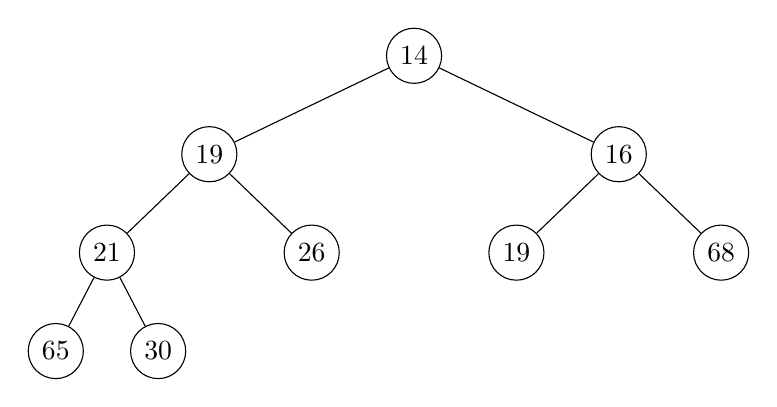
\begin{tikzpicture}[
  level distance=1.25cm,
  level 1/.style={sibling distance=5.2cm},
  level 2/.style={sibling distance=2.6cm},
  level 3/.style={sibling distance=1.3cm},
  every node/.style={circle, draw, minimum size=7mm, inner sep=1pt},
  edge from parent/.style={draw,-}
]
\node {14}
  child { node {19}
    child { node {21}
      child { node {65} }
      child { node {30} }
    }
    child { node {26} }
  }
  child { node {16}
    child { node {19} }
    child { node {68} }
  };
\end{tikzpicture}
\end{center}

\textbf{Step 2: append 17 at index 10}

\[
[\text{EMPTY},\ 14,\ 19,\ 16,\ 21,\ 26,\ 19,\ 68,\ 65,\ 30,\ 17]
\]

\begin{center}
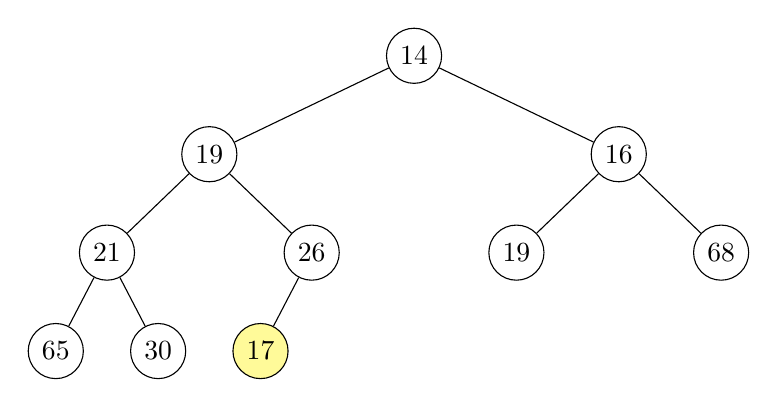
\begin{tikzpicture}[
  level distance=1.25cm,
  level 1/.style={sibling distance=5.2cm},
  level 2/.style={sibling distance=2.6cm},
  level 3/.style={sibling distance=1.3cm},
  level 4/.style={sibling distance=0.9cm},
  every node/.style={circle, draw, minimum size=7mm, inner sep=1pt},
  edge from parent/.style={draw,-}
]
\node {14}
  child { node {19}
    child { node {21}
      child { node {65} }
      child { node {30} }
    }
    child { node {26}
      child { node[fill=yellow!40] {17} }
      child[missing] {}
    }
  }
  child { node {16}
    child { node {19} }
    child { node {68} }
  };
\end{tikzpicture}
\end{center}

\textbf{Step 3: swap with parent 26 at index 5}

\[
[\text{EMPTY}, 14,19,16,21,17,19,68,65,30,26]
\]

\begin{center}
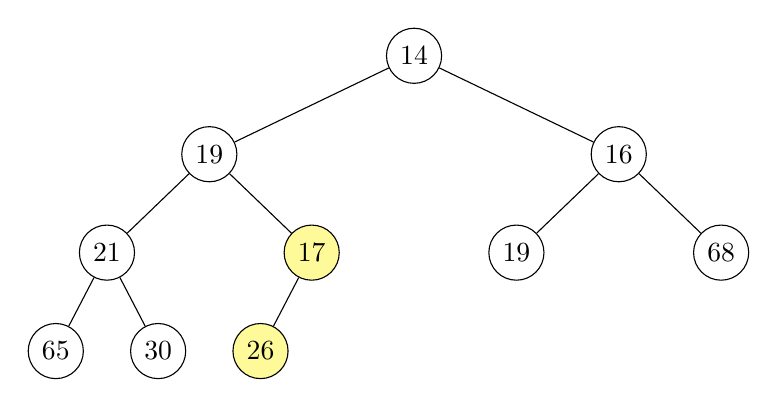
\begin{tikzpicture}[
  level distance=1.25cm,
  level 1/.style={sibling distance=5.2cm},
  level 2/.style={sibling distance=2.6cm},
  level 3/.style={sibling distance=1.3cm},
  level 4/.style={sibling distance=0.9cm},
  every node/.style={circle, draw, minimum size=7mm, inner sep=1pt},
  edge from parent/.style={draw,-}
]
\node {14}
  child { node {19}
    child { node {21}
      child { node {65} }
      child { node {30} }
    }
    child { node[fill=yellow!40] {17}
      child { node[fill=yellow!40] {26} }
      child[missing] {}
    }
  }
  child { node {16}
    child { node {19} }
    child { node {68} }
  };
\end{tikzpicture}
\end{center}

\textbf{Step 4: swap with parent 19 at index 2}

\[
[\text{EMPTY}, 14,17,16,21,19,19,68,65,30,26]
\]

\begin{center}
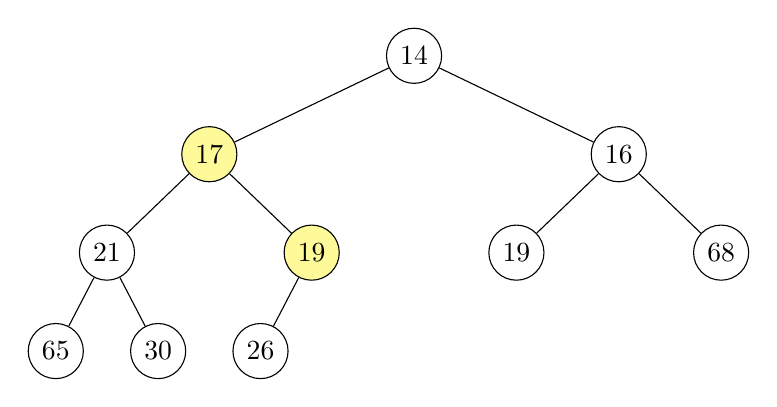
\begin{tikzpicture}[
  level distance=1.25cm,
  level 1/.style={sibling distance=5.2cm},
  level 2/.style={sibling distance=2.6cm},
  level 3/.style={sibling distance=1.3cm},
  level 4/.style={sibling distance=0.9cm},
  every node/.style={circle, draw, minimum size=7mm, inner sep=1pt},
  edge from parent/.style={draw,-}
]
\node {14}
  child { node[fill=yellow!40] {17}
    child { node {21}
      child { node {65} }
      child { node {30} }
    }
    child { node[fill=yellow!40] {19}
      child { node {26} }
      child[missing] {}
    }
  }
  child { node {16}
    child { node {19} }
    child { node {68} }
  };
\end{tikzpicture}
\end{center}

\textbf{Step 5: stop (Index 2 $>$ Index 1, $17 > 14$)}

Final heap:
\[
[\text{EMPTY}, 14,17,16,21,19,19,68,65,30,26]
\]
\textbf{Code:}
\begin{verbatim}
void push(int val) {
    heap.add(val);
    int i = heap.size() - 1;

    while (i > 1 && heap.get(i) < heap.get(i / 2)) {
        int temp = heap.get(i);
        heap.set(i, heap.get(i / 2));
        heap.set(i / 2, temp);
        i = i / 2;
    }
}
\end{verbatim}

\textbf{Time Complexity:} $O(\log n)$

\subsection{Pop (Remove Min)}

To pop from a min-heap:
\begin{itemize}
  \item Replace the root with the last element in the array
  \item Delete the last element
  \item Percolate down: Repeatedly swap the new root with its smaller child while it is larger, moving it downward until both children are larger than or equal to it.
\end{itemize}

\textbf{Step 1: Starting heap}

\[
[\text{EMPTY},\ 14,\ 19,\ 16,\ 21,\ 26,\ 19,\ 68,\ 65,\ 30]
\]

\begin{center}
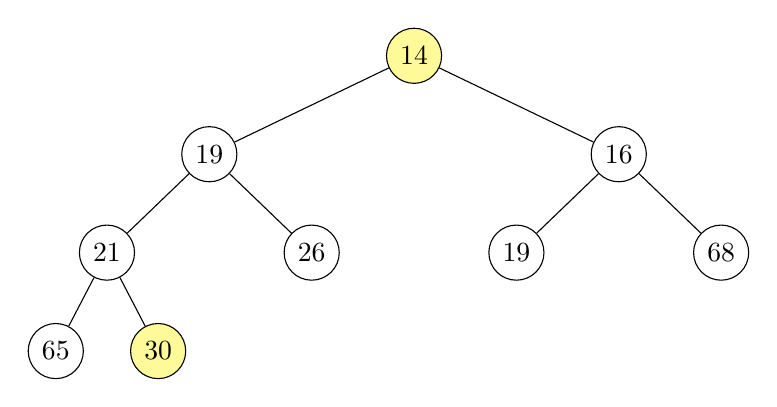
\begin{tikzpicture}[
  level distance=1.25cm,
  level 1/.style={sibling distance=5.2cm},
  level 2/.style={sibling distance=2.6cm},
  level 3/.style={sibling distance=1.3cm},
  every node/.style={circle, draw, minimum size=7mm, inner sep=1pt},
  edge from parent/.style={draw,-}
]
\node[fill=yellow!40] {14}
  child { node {19}
    child { node {21}
      child { node {65} }
      child { node[fill=yellow!40] {30} }
    }
    child { node {26} }
  }
  child { node {16}
    child { node {19} }
    child { node {68} }
  };
\end{tikzpicture}
\end{center}

\textbf{Step 2: swap root with last (30), delete the original root}

\[
[\text{EMPTY}, 30,19,16,21,26,19,68,65]
\]

\begin{center}
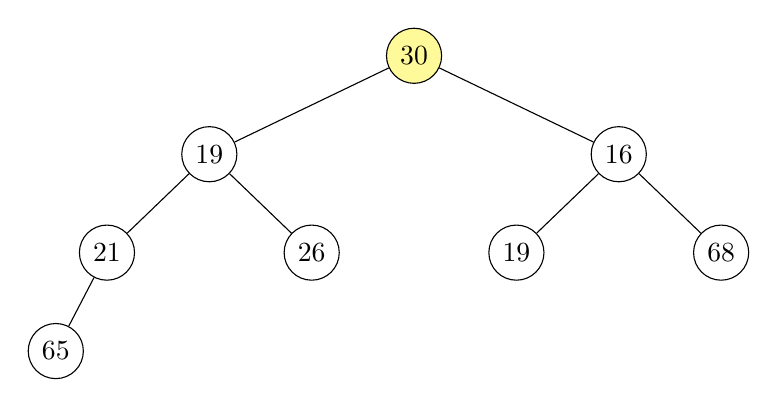
\begin{tikzpicture}[
  level distance=1.25cm,
  level 1/.style={sibling distance=5.2cm},
  level 2/.style={sibling distance=2.6cm},
  level 3/.style={sibling distance=1.3cm},
  every node/.style={circle, draw, minimum size=7mm, inner sep=1pt},
  edge from parent/.style={draw,-}
]
\node[fill=yellow!40] {30}
  child { node {19}
    child { node {21}
      child { node {65} }
      child[missing] {}
    }
    child { node {26} }
  }
  child { node {16}
    child { node {19} }
    child { node {68} }
  };
\end{tikzpicture}
\end{center}

\textbf{Step 3: percolate down, swapping with the smaller child (16)}

\[
[\text{EMPTY}, 16,19,30,21,26,19,68,65]
\]

\begin{center}
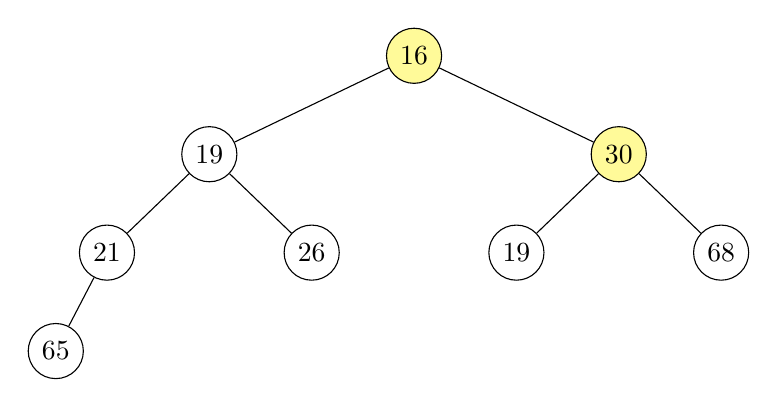
\begin{tikzpicture}[
  level distance=1.25cm,
  level 1/.style={sibling distance=5.2cm},
  level 2/.style={sibling distance=2.6cm},
  level 3/.style={sibling distance=1.3cm},
  every node/.style={circle, draw, minimum size=7mm, inner sep=1pt},
  edge from parent/.style={draw,-}
]
\node[fill=yellow!40] {16}
  child { node {19}
    child { node {21}
      child { node {65} }
      child[missing] {}
    }
    child { node {26} }
  }
  child { node[fill=yellow!40] {30}
    child { node {19} }
    child { node {68} }
  };
\end{tikzpicture}
\end{center}

\textbf{Step 4: swap with smaller child (19)}

\[
[\text{EMPTY}, 16,19,19,21,26,30,68,65]
\]

\begin{center}
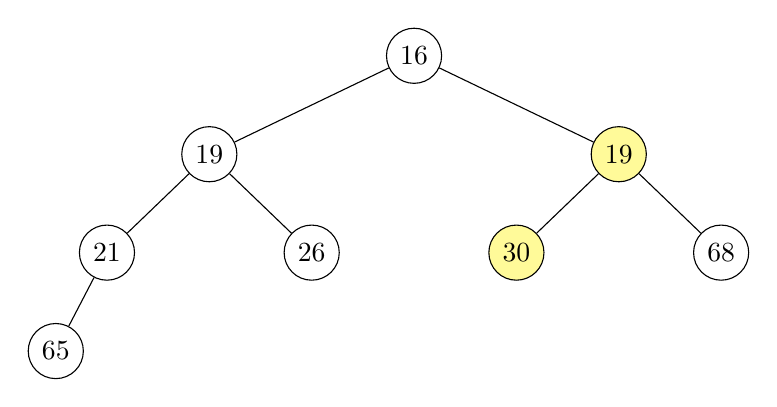
\begin{tikzpicture}[
  level distance=1.25cm,
  level 1/.style={sibling distance=5.2cm},
  level 2/.style={sibling distance=2.6cm},
  level 3/.style={sibling distance=1.3cm},
  every node/.style={circle, draw, minimum size=7mm, inner sep=1pt},
  edge from parent/.style={draw,-}
]
\node {16}
  child { node {19}
    child { node {21}
      child { node {65} }
      child[missing] {}
    }
    child { node {26} }
  }
  child { node[fill=yellow!40] {19}
    child { node[fill=yellow!40] {30} }
    child { node {68} }
  };
\end{tikzpicture}
\end{center}

Final heap:
\[
[\text{EMPTY}, 16,19,19,21,26,30,68,65]
\]
\textbf{Code:}
\begin{verbatim}
int pop() {
    int res = heap.get(1);
    heap.set(1, heap.get(heap.size() - 1));
    heap.remove(heap.size() - 1);

    int i = 1;
    while (2 * i < heap.size()) {
        int smallest = 2 * i;
        if (2 * i + 1 < heap.size()
                && heap.get(2 * i + 1) < heap.get(2 * i))
            smallest = 2 * i + 1;

        if (heap.get(i) > heap.get(smallest)) {
            int temp = heap.get(i);
            heap.set(i, heap.get(smallest));
            heap.set(smallest, temp);
            i = smallest;
        } else break;
    }
    return res;
}
\end{verbatim}

\textbf{Time Complexity:} $O(\log n)$

\subsection{Heapify (Build Heap in $O(n)$)}
Heapify builds a heap from an unsorted array more efficiently than repeated inserts.

\textbf{Step 1: Starting array (unsorted)}
\[
[\text{EMPTY}, 50,80,40,30,10,70,20,90,60]
\]
\begin{center}
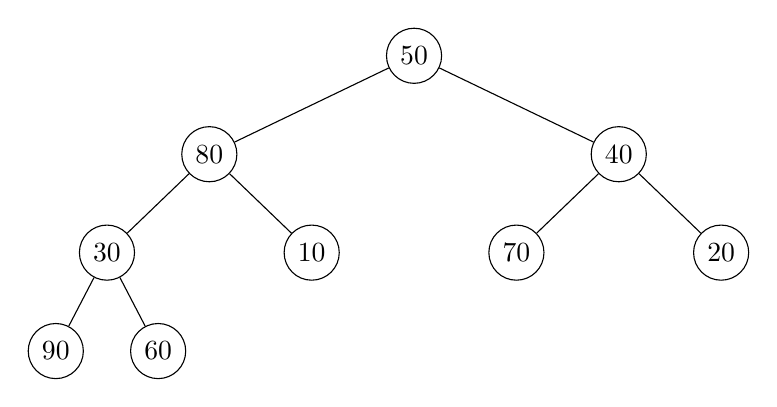
\begin{tikzpicture}[
  level distance=1.25cm,
  level 1/.style={sibling distance=5.2cm},
  level 2/.style={sibling distance=2.6cm},
  level 3/.style={sibling distance=1.3cm},
  every node/.style={circle, draw, minimum size=7mm, inner sep=1pt},
  edge from parent/.style={draw,-}
]
\node {50}
  child { node {80}
    child { node {30}
      child { node {90} }
      child { node {60} }
    }
    child { node {10} }
  }
  child { node {40}
    child { node {70} }
    child { node {20} }
  };
\end{tikzpicture}
\end{center}
Heapify starts at $i = \lfloor n/2 \rfloor = 4$ (node 30), the last node with children (left child = $2i$), and percolates down to the root.

\textbf{Step 2: Process node at index 4 (value 30)}

30 has children 90 and 60. Since $30 < 60$ and $30 < 90$, no swap needed.
\[
[\text{EMPTY}, 50,80,40,30,10,70,20,90,60]
\]
\begin{center}
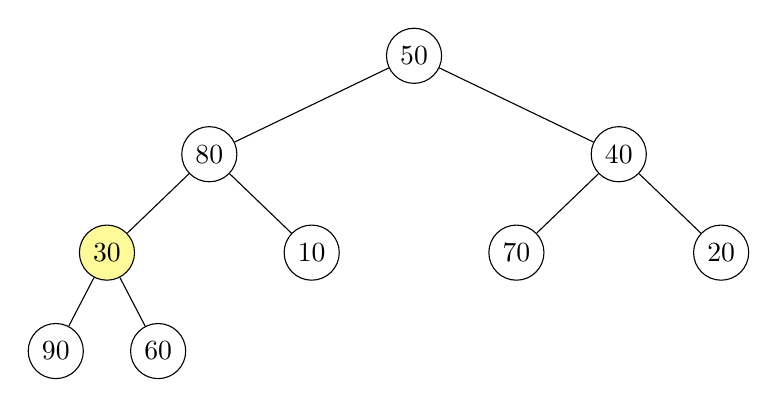
\begin{tikzpicture}[
  level distance=1.25cm,
  level 1/.style={sibling distance=5.2cm},
  level 2/.style={sibling distance=2.6cm},
  level 3/.style={sibling distance=1.3cm},
  every node/.style={circle, draw, minimum size=7mm, inner sep=1pt},
  edge from parent/.style={draw,-}
]
\node {50}
  child { node {80}
    child { node[fill=yellow!40] {30}
      child { node {90} }
      child { node {60} }
    }
    child { node {10} }
  }
  child { node {40}
    child { node {70} }
    child { node {20} }
  };
\end{tikzpicture}
\end{center}

\textbf{Step 3: Process node at index 3 (value 40)}

40 has children 70 and 20. Smaller child is 20. Since $40 > 20$, swap 40 and 20.
\[
[\text{EMPTY}, 50,80,20,30,10,70,40,90,60]
\]
\begin{center}
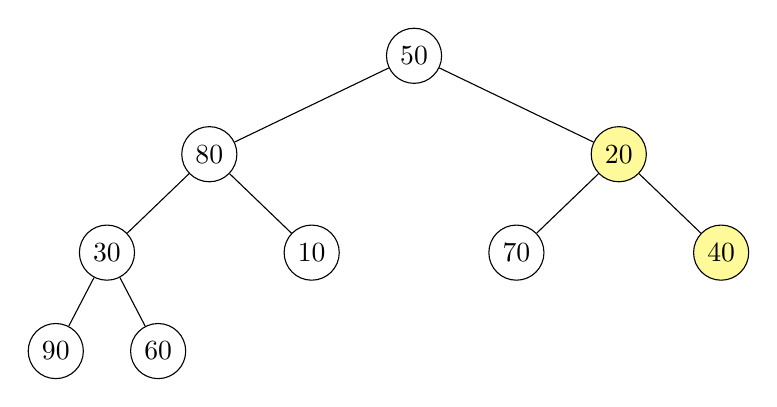
\begin{tikzpicture}[
  level distance=1.25cm,
  level 1/.style={sibling distance=5.2cm},
  level 2/.style={sibling distance=2.6cm},
  level 3/.style={sibling distance=1.3cm},
  every node/.style={circle, draw, minimum size=7mm, inner sep=1pt},
  edge from parent/.style={draw,-}
]
\node {50}
  child { node {80}
    child { node {30}
      child { node {90} }
      child { node {60} }
    }
    child { node {10} }
  }
  child { node[fill=yellow!40] {20}
    child { node {70} }
    child { node[fill=yellow!40] {40} }
  };
\end{tikzpicture}
\end{center}

40 has no children, so we can stop percolating down.

\textbf{Step 4: Process node at index 2 (value 80)}

80 has children 30 and 10. Smaller child is 10. Since $80 > 10$, swap 80 and 10.
\[
[\text{EMPTY},50,10,20,30,80,70,40,90,60]
\]
\begin{center}
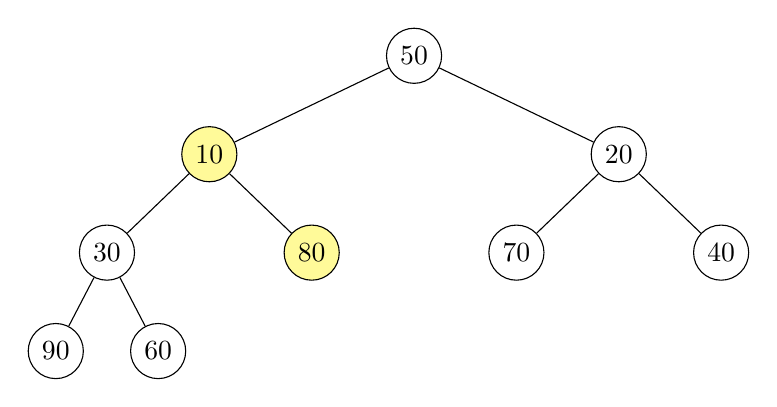
\begin{tikzpicture}[
  level distance=1.25cm,
  level 1/.style={sibling distance=5.2cm},
  level 2/.style={sibling distance=2.6cm},
  level 3/.style={sibling distance=1.3cm},
  every node/.style={circle, draw, minimum size=7mm, inner sep=1pt},
  edge from parent/.style={draw,-}
]
\node {50}
  child { node[fill=yellow!40] {10}
    child { node {30}
      child { node {90} }
      child { node {60} }
    }
    child { node[fill=yellow!40] {80} }
  }
  child { node {20}
    child { node {70} }
    child { node {40} }
  };
\end{tikzpicture}
\end{center}

80 has no children, so we can stop percolating down.

\textbf{Step 5: Process node at index 1 (value 50, the root)}

50 has children 10 and 20. Smaller child is 10. Since $50 > 10$, swap 50 and 10.
\[
[\text{EMPTY},10,50,20,30,80,70,40,90,60]
\]
\begin{center}
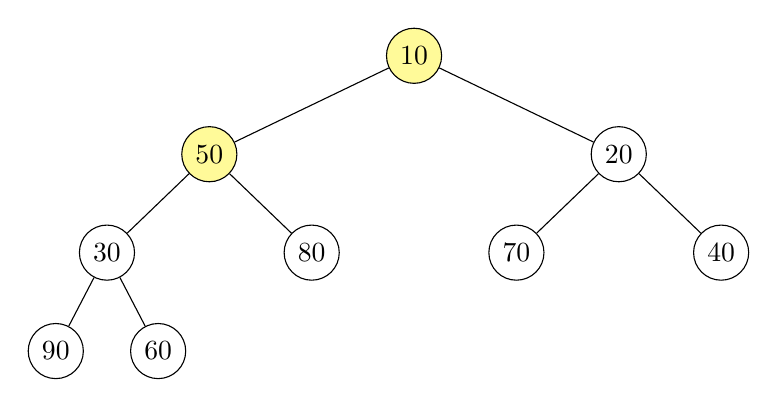
\begin{tikzpicture}[
  level distance=1.25cm,
  level 1/.style={sibling distance=5.2cm},
  level 2/.style={sibling distance=2.6cm},
  level 3/.style={sibling distance=1.3cm},
  every node/.style={circle, draw, minimum size=7mm, inner sep=1pt},
  edge from parent/.style={draw,-}
]
\node[fill=yellow!40] {10}
  child { node[fill=yellow!40] {50}
    child { node {30}
      child { node {90} }
      child { node {60} }
    }
    child { node {80} }
  }
  child { node {20}
    child { node {70} }
    child { node {40} }
  };
\end{tikzpicture}
\end{center}

\textbf{Step 6: Continue percolating the original root down}

50 has children 30 and 80. Smaller child is 30. Since $50 > 30$, swap 50 and 30.
\[
[10,30,20,50,80,70,40,90,60]
\]
\begin{center}
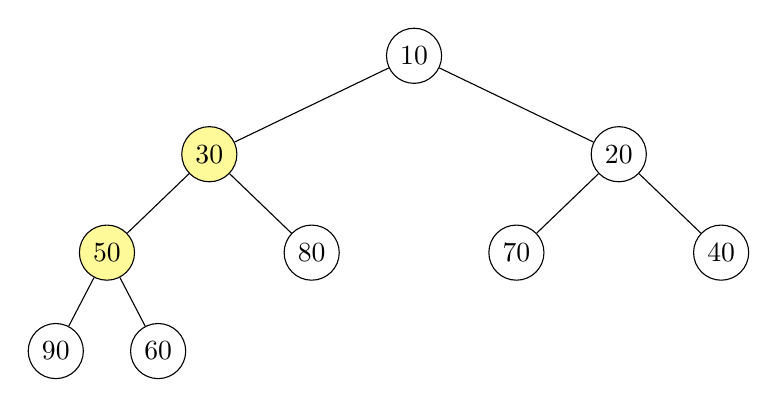
\begin{tikzpicture}[
  level distance=1.25cm,
  level 1/.style={sibling distance=5.2cm},
  level 2/.style={sibling distance=2.6cm},
  level 3/.style={sibling distance=1.3cm},
  every node/.style={circle, draw, minimum size=7mm, inner sep=1pt},
  edge from parent/.style={draw,-}
]
\node {10}
  child { node[fill=yellow!40] {30}
    child { node[fill=yellow!40] {50}
      child { node {90} }
      child { node {60} }
    }
    child { node {80} }
  }
  child { node {20}
    child { node {70} }
    child { node {40} }
  };
\end{tikzpicture}
\end{center}

\textbf{Step 7: Continue percolating 50 down}

50 has children 90 and 60. Smaller child is 60. Since $50 < 60$, stop. Heap property satisfied.

\textbf{Final heap:}
\[
[10,30,20,50,80,70,40,90,60]
\]
\begin{center}
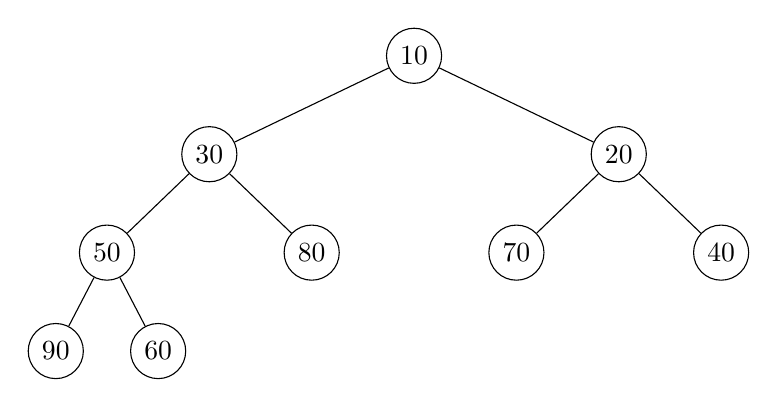
\begin{tikzpicture}[
  level distance=1.25cm,
  level 1/.style={sibling distance=5.2cm},
  level 2/.style={sibling distance=2.6cm},
  level 3/.style={sibling distance=1.3cm},
  every node/.style={circle, draw, minimum size=7mm, inner sep=1pt},
  edge from parent/.style={draw,-}
]
\node {10}
  child { node {30}
    child { node {50}
      child { node {90} }
      child { node {60} }
    }
    child { node {80} }
  }
  child { node {20}
    child { node {70} }
    child { node {40} }
  };
\end{tikzpicture}
\end{center}
\textbf{Code:}
\begin{verbatim}
void heapify(List<Integer> a) {
    a.add(0, 0); // dummy for 1-based indexing
    for (int i = (a.size() - 1) / 2; i >= 1; i--) {
        int j = i;
        while (2 * j < a.size()) {
            int c = 2 * j;
            if (c + 1 < a.size() && a.get(c + 1) < a.get(c))
                c++;
            if (a.get(j) > a.get(c)) {
                int temp = a.get(j);
                a.set(j, a.get(c));
                a.set(c, temp);
                j = c;
            } else break;
        }
    }
}
\end{verbatim}

Heapify is $O(n)$ because most nodes are near the bottom and percolate down only a few levels, while the few nodes near the top that percolate far down are outnumbered.

\subsection{Time Complexities}
\begin{center}
\begin{tabular}{l c}
\toprule
Operation & Time \\
\midrule
Get Min / Max & $O(1)$ \\
Push & $O(\log n)$ \\
Pop & $O(\log n)$ \\
Heapify & $O(n)$ \\
\bottomrule
\end{tabular}
\end{center}